\section{Anatomy}\label{sec:anatomy}

\begin{wrapfigure}{R}{0.3\textwidth}
    \centering
    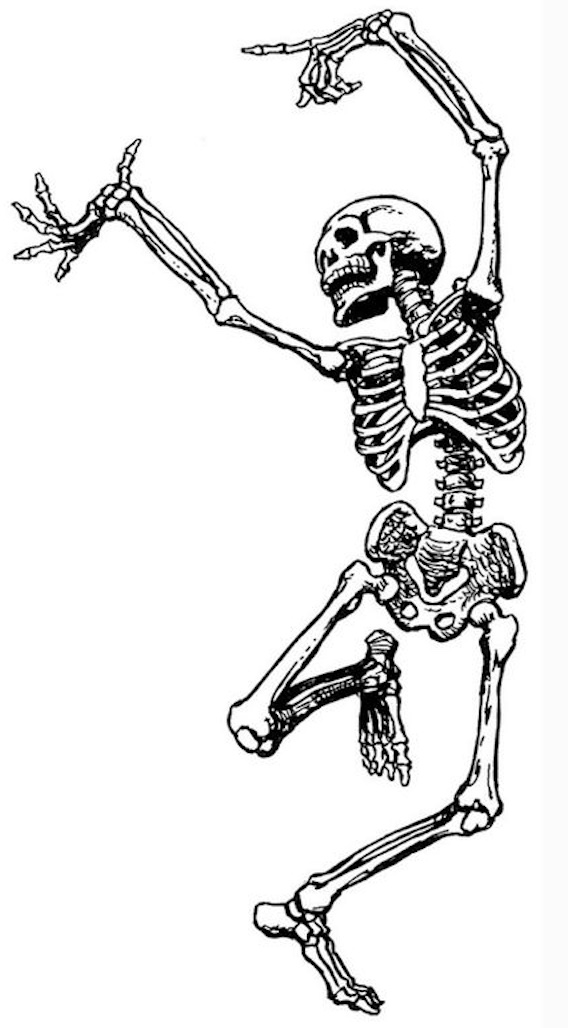
\includegraphics[width=0.25\textwidth]{images/anatomy}
\end{wrapfigure}

As with every system dealing with the human body, a basic understanding of the human anatomical body is mandatory, adding a tremendous benefit for the practice, and also becomes handy when communicating certain aspects to others.
The field of anatomy is of course huge and doesn't need to be studied in-depth.
Yet, you should make yourself familiar with some hand-picked medical terms and the basic concepts of the human body to also have a theoretical understanding of what's happening during the dance.

\subsection{Terminology}\label{subsec:terminology}

In order to understand the following, it is mandatory to be familiar with some basic terms used in medical anatomy.

\subsubsection{Orientation}

\begin{itemize}
    \setlength\itemsep{0em}
    \item anterior/posterior = front/back
    \item ventral/dorsal = front/back of the torso
    \item superior/inferior = above/below
    \item cranial/caudal = head-/tail-wards
    \item proximal/distal = towards to/away from center
    \item medial/lateral = towards/away the midline
    \item superficial/profund = more away/inside the body
\end{itemize}

\subsubsection{Movements}

\begin{itemize}
    \setlength\itemsep{0em}
    \item extension/flexion = making the angle of a joint (elbow, knee) bigger/smaller
    \item internal/external rotation = straight arm/leg rotating in the shoulder/hip join; alias medial/lateral rotation
    \item adduction/abduction = moving towards or away the body/midline
    \item elevation/depression = moving superior/inferior direction (e.g. shoulder shrug/lowering)
    \item pronation/supination = forearm rotating palm down/palm up (not same as rotation)
    \item dorsi-/plantarflexion = ankle only; moving towards the dorsum (superior surface) or plantar (sole) alias ``point''
    \item in-/eversion = ankle only; sole towards/away the median plane, so they face medial/lateral direction
    \item opposition/reposition = thumb and little finger together/away from each other
    \item circumduction = conical (not really circular) movement of a limb extending from the joint its moved by
    \item pro-/retraction = anterolateral/posteromedial movement of scapula (move shoulder forward/backward)
\end{itemize}

Terms derived from lateral include:

\begin{itemize}
    \setlength\itemsep{0em}
    \item Uni-lateral = unus meaning ``one'', on one side of the body, e.g. just one leg.
    \item Bi-lateral = bis meaning ``twice'', on both sides of the body, e.g. both legs.
    \item Homo-lateral (Ipsi-lateral) = ipse meaning ``same'', e.g. using the arm and leg of the same side.
    \item Contra-lateral = contra meaning ``against'', e.g. arm one side and other side leg creating an X-shape, like we do in walking (also one side of brain hemisphere is controlling other side of the body).
\end{itemize}

Sometimes the latin word for left (sinister) and right (dexter) are used.

\subsection{Structures}\label{subsec:structures}

\subsubsection{Bones}

The whole human body (usually) consists of 206 bones; yet by birth we have a few more which results to 280.
80 bones are part of the head and trunk (axial skeleton) and 126 make up the limbs (appendicular skeleton).

There are 27 bones for each hand (19 for phalanges+metacarpals and 8 carpals), and 26 for each foot (phalanges, metatarsals, and tarsals).

\begin{itemize}
    \setlength\itemsep{0em}
    \item atlas and axis = two top most cervical vertebra
    \item clavicle = collar bone
    \item coccyx = tailbone (last part of the sacrum)
    \item cranium = skull (cervical = neck)
    \item patella = kneecap
    \item processus = a bony thing bulging out, usually for tendons to attach to
    \item ribs = true (1-7, sternum connection), false (8-10/12, cartilage), floating (11-12, no connection)
    \item scapula = shoulder blade
    \item SIAS = Spina Illiaca Anterior Superior (front top pointy bone structure of the pelvis)
    \item spina = spine (consisting of 33 vertebrae: 7 cervical, 12 thoracic, 5 lumbar, 5 fused sacrum, 4 fused coccyx)
    \item sternum = chest bone
\end{itemize}

\subsubsection{Muscles}

There are between 600 and 840 muscles within the typical human body, depending on how they are counted.

\begin{itemize}
    \setlength\itemsep{0em}
    \item abs = abdominal muscles (3 layers of different muscles wrapped around the belly)
    \item core muscles = basically everything attached to the spine (not only the abs)
    \item diaphragm = muscle for breathing bottom of ribs
    \item glutes = buttocks (three parts: maximus, medius, minimus)
    \item obliques = part of the core, sides of the abs
    \item pectoralis = chest muscle
    \item pelvic floor = similar to diaphragm but at the bottom of the torso
    \item stomach muscles = the stomach is an organ, which indeed has muscles, but it's located on the left side underneath the ribs, and should not be confused with abs / lower belly!
    \item trapezius = top shoulder around the neck
    \item transverse = part of the core, like a belt around it
\end{itemize}

\subsection{Planes}\label{subsec:planes}

\begin{wrapfigure}{R}{0.3\textwidth}
    \centering
    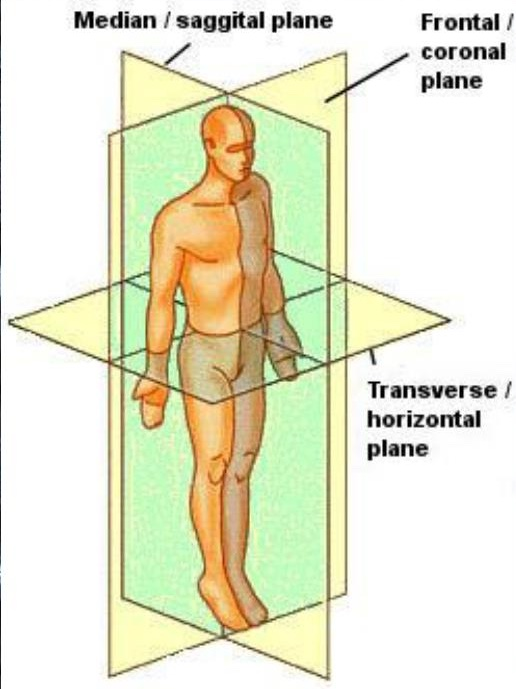
\includegraphics[width=0.25\textwidth]{images/anatomy_planes}
    \caption{The three anatomic planes for the human body: Frontal, Sagittal and Transversal.}
\end{wrapfigure}

We differentiate three different anatomical planes in which movement can happen:

\begin{enumerate}
    \setlength\itemsep{0em}
    \item \textbf{Frontal Plane}: Also called \textit{Coronal Plane} or \textit{Vertical Plane} and, not surprisingly, represents the plane when looking from the front of the body, dividing the body in an anterior/posterior part.
    The directions can be medial/lateral thus resulting in the movements of: ad-/abduction, elevation/depression and in-/eversion.
    \item \textbf{Sagittal Plane}: Also called \textit{Lateral Plane}, \textit{Longitudinal Plane} or \textit{Anteroposterior Plane}, which is going through the midline and shows the body when looking from the side, separating it into a left/right part.
    The directions are thus anterior/posterior and movements are flexion/extension and pro-/retraction.
    \item \textbf{Transverse Plane}: Also called \textit{Axial Plane}, \textit{Horizontal Plane} (the other two planes are vertical) or \textit{Cross-Sectional Plane}, and divides the body into a top/bottom part.
    Directions are thus superior/inferior and allowing movements like rotation, supination/pronation and circumduction.
\end{enumerate}

\subsection{Joints}\label{subsec:joints}

Bones are connected through joints where muscles (together with tendons) can evoke movement.
For different movements, different types of (synovial) joints are needed.

\begin{itemize}
    \setlength\itemsep{0em}
    \item Ball/Socket: hip, shoulder; free movement
    \item Pivot: head (atlantoaxial), elbow (radioulnar); rotation only
    \item Hinge: elbow (humeroulnar), knee, ankle; usually flexion/extension
    \item Saddle: fingers-hand (trapeziometacarpal)
    \item Condyloid: between fingers/wrist (metacarpophalangeal)
    \item Plane: hand (intercarpal) and feet (tarsal)
    \item Gliding: Foot mini bones
\end{itemize}
